\documentclass[12pt]{article}
\usepackage{amsmath}
\usepackage{graphicx}
\usepackage{listings}
\usepackage{amsfonts}
\usepackage{amssymb}
\usepackage{hyperref}
\usepackage{tocloft}

\title{Problem Sheet 1 Answer}
\author{Junbiao Li - 209050796}
\date{\today}

\renewcommand{\cftsecleader}{\cftdotfill{\cftdotsep}}  % 对于 \section
\renewcommand{\cftsubsecleader}{\cftdotfill{\cftdotsep}}  % 对于 \subsection

\begin{document}

\maketitle
\tableofcontents


\clearpage
\section{Problem 1}

Let $x_G$ be the production volume of Growrite (G) in liters, and \( x_T \) be the production volume of Tomfood (T) in liters.

Each type of fertilizer requires three basic ingredients (N, P, K), and there is a limited amount of these ingredients available each day.
\begin{itemize}
    \item  For Nitrogen (N), Growrite requires 0.11 kg/L and Tomfood requires 0.08 kg/L. A total of 600 kg is available.
    
    \[ 0.11 \cdot x_G + 0.08 \cdot x_T \leq 600 \]
    
    \item  For Phosphorus (P), Growrite requires 0.06 kg/L and Tomfood requires 0.03 kg/L. A total of 300 kg is available.
    
    \[ 0.06 \cdot x_G + 0.03 \cdot x_T \leq 300 \]
    
    \item  For Potassium (K), Growrite requires 0.02 kg/L and Tomfood requires 0.08 kg/L. A total of 330 kg is available.
    
    \[ 0.02 \cdot x_G + 0.08 \cdot x_T \leq 330 \]
    
\end{itemize}
    
Biocare aims to maximize its daily income. The selling price for Growrite is £2.80/L, and for Tomfood, it's £3.00/L.

\[ \max Z = 2.80 \cdot x_G + 3.00 \cdot x_T \]


Combining all the information, we have the following linear programming problem:

\[
\begin{array}{cc}
 \max & Z = 2.80 \cdot x_G + 3.00 \cdot x_T \\
\text { s.t. } & 0.11 \cdot x_G + 0.08 \cdot x_T \leq 600 \\
& 0.06 \cdot x_G + 0.03 \cdot x_T \leq 300 \\
& 0.02 \cdot x_G + 0.08 \cdot x_T \leq 330 \\
& x_G, x_T \geq 0 \\
\end{array}
\]

\clearpage
\section{Problem 2}

After solving linear programming problem:

\begin{figure}[h]
    \centering
    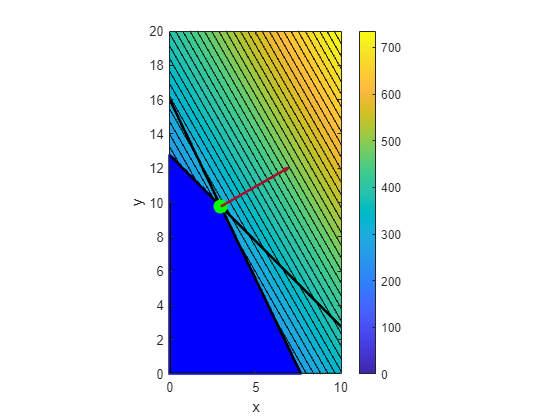
\includegraphics[width=0.5\textwidth]{fig1.png}
    \caption{}
    \label{fig:figa}
\end{figure}

It can be seen from the figure~\ref{fig:figa} that only constraint $23 x+11 y \leq 176$ and constraint $4 x+4 y \leq 51$ are active, since the direction of the gradient is toward the upper right corner of the image.

\subsection{MATLAB Code}
\begin{lstlisting}[language=Matlab, basicstyle=\scriptsize]
clear, close all;

% Define the coefficients for the objective function
f = [-35; -20];  % Note the negative signs for a maximization problem


% Define the inequality constraint matrix and vector
A = [23, 11; 4, 4];
b = [176; 51];

% Define the lower bound for the variables
lb = [0; 0];

% Create optimization options
options = optimoptions('linprog', 'Display', 'none');

% Solve the linear programming problem
[x, fval, exitflag, output] = linprog(f, A, b, [], [], lb, [], options);

% Convert the objective function value back to the original maximization problem
optimal_value = -fval;

% Display the results
fprintf('The optimal solution is x = %f, y = %f\n', x(1), x(2));
fprintf('The maximum value of the objective function is %f\n', optimal_value);
\end{lstlisting}

\clearpage
\section{Problem 3}
\begin{enumerate}
    
    \item  For the first constraint \(3x - 7z \leq 176\), which is equivalent to \(3x - 7z + s_1 = 176\) where, \(s_1 \geq 0\).
    
    \item For the second constraint \(8z - 2y + x - 6 \geq 12\), We have \(8z - 2y + x - 6 - s_2 = 12\) where, \(s_2 \geq 0\).
    
    \item The third constraint \(4x + 3y = 19\) is already an equality constraint and needs no change.
    
    \item Using new variables \(x_+, x_-, y_+, y_-, z_+, z_-\) to represent the positive and negative parts of \(x, y, z\), respectively. Specifically, \(x = x_+ - x_-\), \(y = y_+ - y_-\), \(z = z_+ - z_-\), where \(x_+, x_-, y_+, y_-, z_+, z_- \geq 0\).
\end{enumerate}

Letting \( \mathbf{x} \) = \([x_+, x_-, y_+, y_-, z_+, z_-, s]^T\), hence

\[
\begin{array}{lll}
\text{max} & \begin{pmatrix} -30 & 30 & -21 & 21 & -18 & 18 & 0 \end{pmatrix} \begin{pmatrix} x_+ \\ x_- \\ y_+ \\ y_- \\ z_+ \\ z_- \\ s \end{pmatrix} & \\
\text{s.t.} & \begin{pmatrix}
3 & -3 & 0 & 0 & -7 & 7 & 0 \\
-1 & 1 & 2 & -2 & -8 & 8 & 0 \\
4 & -4 & 3 & -3 & 0 & 0 & -1 \\
-4 & 4 & -3 & 3 & 0 & 0 & 1
\end{pmatrix} \begin{pmatrix} x_+ \\ x_- \\ y_+ \\ y_- \\ z_+ \\ z_- \\ s \end{pmatrix} \leq \begin{pmatrix} 176 \\ -12 \\ 19 \\ -19 \end{pmatrix} & \\
& \begin{pmatrix} x_+ \\ x_- \\ y_+ \\ y_- \\ z_+ \\ z_- \\ s \end{pmatrix} \geq \begin{pmatrix} 0 \\ 0 \\ 0 \\ 0 \\ 0 \\ 0 \\ 0 \end{pmatrix} &
\end{array}
\]

\clearpage
\section{Problem 4}

First, we have the primal problem:

\[
\begin{array}{cc}
\min & \left( \begin{array}{ccc} 1 & 4 & -9 \end{array} \right) z \\
\text { s.t. } & \left( \begin{array}{ccc} 1 & 0 & -1 \\ 1 & 1 & 1 \\ 4 & 3 & 0 \end{array} \right) z = \left( \begin{array}{c} 7 \\ 2 \\ 19 \end{array} \right) \\
& x, y, z \geq 0
\end{array}
\]

To obtain its dual, we introduce the Lagrange multipliers y and construct the **Lagrangian Function**:

\[ L(z,y) = \left( \begin{array}{ccc} 1 & 4 & -9 \end{array} \right) z + y^T \left( \left( \begin{array}{c} 7 \\ 2 \\ 19 \end{array} \right) - \left( \begin{array}{ccc} 1 & 0 & -1 \\ 1 & 1 & 1 \\ 4 & 3 & 0 \end{array} \right) z \right)  - s^T z
\]

Next, to obtain the **Dual Function**, we minimize the Lagrangian with respect to z:

\[
\begin{aligned}
g(y) &= \min_{z} L(z,y)  \\
&= \min_{z} z^T \left( \left( \begin{array}{c} 1 \\ 4 \\ -9 \end{array} \right) + y^T \left(\begin{array}{rrr}
1 & 1 & 4 \\
0 & 1 & 3 \\
-1 & 1 & 0
\end{array}\right) \right)  + \left( \begin{array}{c} 7 \\ 2 \\ 19 \end{array} \right)^T y 
\end{aligned}
\]

Based on the above dual function, we can form the \textbf{Dual Problem}:
$$
\begin{array}{cc}
\max & \left( \begin{array}{ccc} 7 & 2 & 19 \end{array} \right) y \\
\text { s.t. } & \left( \begin{array}{c} 1 \\ 4 \\ -9 \end{array} \right) - \left(\begin{array}{rrr}
1 & 1 & 4 \\
0 & 1 & 3 \\
-1 & 1 & 0
\end{array}\right) y = s \\
& s \geq 0,y \in \mathbb{R}^3
\end{array}
$$
    
\clearpage
\section{Problem 5}
\[
\begin{array}{cc}
 \max & \ x_1 + x_2 \\
\text { s.t. } &  \|x\|_1^2 \leq 4 \\
\end{array}
\]

which is equivalent to:

\[
\begin{array}{cc}
 \max & \ x_1 + x_2 \\
\text { s.t. } &  \|x\|_1 \leq 2 \\
\end{array}
\]

With auxiliary variables \(z_1\) and \(z_2\), transforming the problem into:
\[
\begin{array}{cc}
 \max & \ x_1 + x_2 \\
\text { s.t. } & |x_1| \leq z_1\\
& |x_2| \leq z_2\\
& z_1 + z_2 = 2\\
\end{array}
\]

\clearpage
\section{Problem 6}
$$
\begin{gathered}
\min \quad z_1+z_2+\cdots+z_n \\
\text { s.t. }-z \leq w \leq z \\
A w=y . \\
w, z \in \mathbb{R}^n
\end{gathered}
$$
To make $z_1+z_2+\cdots+z_n$ is desired to be minimal, since A have full rank which means $w$ is unique, we can let 
Let
$$
\begin{gathered}
0 \leq|w| \leq z \\
0 \leq\left|w_1\right| \leq z_1 \\
\quad \cdots \\
0 \leq\left|w_n\right| \leq z_n
\end{gathered}
$$
Therefore, when $z_1=w_1, z_2=w_2, \cdots, z_n=w_n \leftrightarrow z=|w|$ which satisfies $A w=y$
Hence, that $z^*=\left|w^*\right|$.


\clearpage
\section{Problem 7}
\begin{figure}[h]
    \centering
    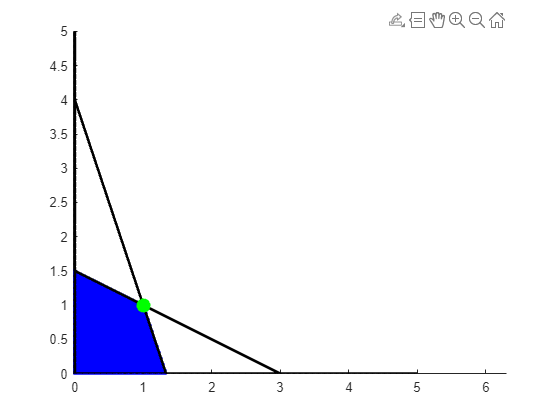
\includegraphics[width=0.5\textwidth]{fig2.png}
    % \caption{Your caption}
    \label{fig:fig2}
\end{figure}

The objective function is to maximize \(c^T x\), where \(c = (\cos(\alpha), \sin(\alpha))^T\). The gradient of this function is \(c\) itself. For \((1,1)\) to be an optimal solution, the gradient \(c\) should point in a direction where the function \(c^T x\) is maximized when starting from \((1,1)\).

The relevant slopes of the boundaries at the vertex \((1, 1)\) are \(-1/2\) and \(-3\). For \((1,1)\) to be an optimal solution, \(\alpha\) should fall between these two angles, i.e., \(\arctan(1/3) \leq \alpha \leq \arctan(2) \). Hence, for \(\alpha \in [0.32, 1.11]\), the point \(x = (1,1)^T\) is an optimal solution to the given linear programming problem.

\clearpage
\section{Problem 8}
Original problem is:
$$\begin{array}{cc}
\max & b^T y \\
\text { s.t. } & c-A^T y=s \\
& s \geq 0, y \in \mathbb{R}^m
\end{array}$$

First we write the **Standard Form**
For the constraint $c-A^T y=s$, we have
$$
\begin{aligned}
& c-A^T y \leq s \\
& c-A^T y \geq-s
\end{aligned}
$$
And $s \geq 0$, we can rewrite as:
$$
\begin{gathered}
A^T y \leq c+s \\
-A^T y \leq s-c
\end{gathered}
$$
For the purpose of writing this in standard form, we introduce the new variable.
Let $y=y_1-y_2$
The standard form is
$$
\begin{array}{cl}
\min & b^T\left(y_1-y_2\right) \\
\text { s.t. } & A^T\left(y_1-y_2\right)=c-s \\
& y_1, y_2 \geq 0
\end{array}
$$

Now we are proving that this problem is infeasible if and only if there is an  $x \geq 0$ such that  $Ax=0$ and  $c^T x<0$

Since this problem is infeasible, which means the feasible set $F_d = \varnothing$.

If the feasible set $F_d \neq \varnothing$, we have 
$$
\begin{aligned}
A^T y + s &= c \\
(A^T y + s)^T x &= c^T x \\
y^T Ax + s^Tx &= c^T x \\
s^T x &= c^T x \quad \text{(Since we assume that $Ax=0$)} \\
\end{aligned}
$$

However, we know that $s \geq 0$ and $c^T x < 0$, which is a contradiction. Hence, the feasible set $F_d = \varnothing$. We prove that this problem is infeasible if there is an $x \geq 0$ such that  $Ax=0$ and  $c^T x<0$.

And we can prove by Farkas' lemma that this problem is infeasible then there is an  $x \geq 0$ such that  $Ax=0$ and  $c^T x<0$.

Hence, we have proved that this problem is infeasible if and only if there is an  $x \geq 0$ such that  $Ax=0$ and  $c^T x<0$.


\clearpage
\section{Problem 9}

optimal soln is $x = (0.00, 3.00)$, $p* = 3.00$

\subsection{MATLAB Code}



\begin{lstlisting}[language=Matlab, basicstyle=\scriptsize]
    f = [1, 1];

    A = [-2, -2; 12, 5];
    b = [-5; 30];
    
    lb = [0, 0];
    ub = [inf, inf];
    
    opts = optimoptions('linprog','Display','none');
    
    intcon = [1, 2];
    [x,fval]= linprog(f,A,b,[],[],lb, ub, opts);
    fprintf("optimal soln is x = (%1.2f, %1.2f), p* = %1.2f\n", [x; fval]) 
    
    %% impose x(2) <= 2
    [x,fval] = linprog(f,A,b,[],[],lb, [inf, 2], opts);
    fprintf("optimal soln with y(2)<=2 is x = (%1.2f, %1.2f), p* = %1.2f\n", [x; fval]) 
    
    %% impose x(2) >= 3
    [x,fval] = linprog(f,A,b,[],[],[0, 3],ub, opts);
    fprintf("optimal soln with y(2)>=3 is x = (%1.2f, %1.2f), p* = %1.2f\n", [x; fval]) 
    
    %% using intlinprog
    opts = optimoptions('intlinprog', 'Display', 'none');
    [x, fval] = intlinprog(f, intcon, A, b, [], [], lb, ub, opts);
    
    fprintf("optimal soln is x = (%1.2f, %1.2f), p* = %1.2f\n", [x; fval]) 
\end{lstlisting}

\clearpage

\appendix
\section*{Appendix}
\addcontentsline{toc}{section}{Appendix}
\renewcommand{\thesubsection}{\Alph{subsection}}

\subsection{MATLAB Code}

\begin{lstlisting}[language=Matlab, basicstyle=\scriptsize]
    %%Problem 2
    clear, close all;
    
    % Define the coefficients for the objective function
    f = [-35; -20];  % Note the negative signs for a maximization problem
    
    % Define the inequality constraint matrix and vector
    A = [23, 11; 4, 4];
    b = [176; 51];
    
    % Define the lower bound for the variables
    lb = [0; 0];
    
    % Create optimization options
    options = optimoptions('linprog', 'Display', 'none');
    
    % Solve the linear programming problem
    [x, fval, exitflag, output] = linprog(f, A, b, [], [], lb, [], options);
    
    % Convert the objective function value back to the original maximization problem
    optimal_value = -fval;
    
    % Display the results
    fprintf('The optimal solution is x = %f, y = %f\n', x(1), x(2));
    fprintf('The maximum value of the objective function is %f\n', optimal_value);
    
    % Create meshgrid for plotting
    [X, Y] = meshgrid(linspace(0, 10, 401), linspace(0, 20, 401));
    
    % Define and plot objective function
    f = @(x,y) 35*x + 20*y;
    contourf(X, Y, f(X,Y), 50); colorbar;
    xlim([0, 10]), ylim([0, 20]), axis equal, hold on;
    
    % Determine and plot feasible region using logical indexing
    idx1 = 23*X + 11*Y <= 176;  % Constraint 1
    idx2 = 4*X + 4*Y <= 51;     % Constraint 2
    idx3 = X >= 0;              % Non-negative constraint for x
    idx4 = Y >= 0;              % Non-negative constraint for y
    
    % Combine all constraints
    idx = idx1 & idx2 & idx3 & idx4;
    
    % Extract coordinates of feasible region
    Xf = X(idx); Yf = Y(idx);
    
    % Plot feasible region
    plot(Xf, Yf, '.b')
    
    % Plot boundary of feasible region
    t = linspace(0, 10, 400);
    lw = 'linewidth';
    plot(t, (176 - 23*t)/11, '-k', lw, 2)  % Constraint boundary 1
    plot(t, (51 - 4*t)/4, '-k', lw, 2)     % Constraint boundary 2
    plot(zeros(size(t)), t, '-k', lw, 2)   % Non-negative constraint for x
    plot(t, zeros(size(t)), '-k', lw, 2)   % Non-negative constraint for y
    
    % Mark the optimal solution
    opt_x = x(1);
    opt_y = x(2);
    plot(opt_x, opt_y, 'go', 'MarkerSize', 10, 'MarkerFaceColor', 'g');
    
    % Plot normalized gradient
    grad_f = [35; 20];
    grad_f = 5*grad_f / norm(grad_f);
    quiver(opt_x, opt_y, grad_f(1), grad_f(2), 'linewidth', 2)
    hold off
    
    %%Problem 7
    clear, close all;
    
    % Define the coefficients for the objective function
    f = [-35; -20];  % Note the negative signs for a maximization problem
    
    % Define the inequality constraint matrix and vector
    A = [23, 11; 4, 4];
    b = [176; 51];
    
    % Define the lower bound for the variables
    lb = [0; 0];
    
    % Create optimization options
    options = optimoptions('linprog', 'Display', 'none');
    
    % Solve the linear programming problem
    [x, fval, exitflag, output] = linprog(f, A, b, [], [], lb, [], options);
    
    % Convert the objective function value back to the original maximization problem
    optimal_value = -fval;
    
    % Display the results
    fprintf('The optimal solution is x = %f, y = %f\n', x(1), x(2));
    fprintf('The maximum value of the objective function is %f\n', optimal_value);
    
    % Create meshgrid for plotting
    [X, Y] = meshgrid(linspace(0, 10, 1001), linspace(0, 10, 1001));
    
    % Define and plot objective function
    %f = @(x,y) 35*x + 20*y;
    %contourf(X, Y, f(X,Y), 50); colorbar;
    xlim([0, 5]), ylim([0, 5]), axis equal, hold on;
    
    % Determine and plot feasible region using logical indexing
    idx1 = X + 2*Y <= 3;  % Constraint 1
    idx2 = 3*X + Y <= 4;     % Constraint 2
    idx3 = X >= 0;              % Non-negative constraint for x
    idx4 = Y >= 0;              % Non-negative constraint for y
    
    % Combine all constraints
    idx = idx1 & idx2 & idx3 & idx4;
    
    % Extract coordinates of feasible region
    Xf = X(idx); Yf = Y(idx);
    
    % Plot feasible region
    plot(Xf, Yf, 'b.')
    
    % Plot boundary of feasible region
    t = linspace(0, 5, 400);
    lw = 'linewidth';
    plot(t, 3/2-t/2, '-k', lw, 2)  % Constraint boundary 1
    plot(t, -3*t+4, '-k', lw, 2)     % Constraint boundary 2
    plot(zeros(size(t)), t, '-k', lw, 2)   % Non-negative constraint for x
    plot(t, zeros(size(t)), '-k', lw, 2)   % Non-negative constraint for y
    
    % Mark the optimal solution
    opt_x = 1;
    opt_y = 1;
    plot(opt_x, opt_y, 'go', 'MarkerSize', 10, 'MarkerFaceColor', 'g');
    
    % Plot normalized gradient
    %grad_f = [35; 20];
    %grad_f = 5*grad_f / norm(grad_f);
    %quiver(opt_x, opt_y, grad_f(1), grad_f(2), 'linewidth', 2)
    
    %%Problem 9
    f = [1, 1];
    
    A = [-2, -2; 12, 5];
    b = [-5; 30];
    
    lb = [0, 0];
    ub = [inf, inf];
    
    opts = optimoptions('linprog','Display','none');
    
    intcon = [1, 2];
    [x,fval]= linprog(f,A,b,[],[],lb, ub, opts);
    fprintf("optimal soln is x = (%1.2f, %1.2f), p* = %1.2f\n", [x; fval]) 
    
    %% impose x(2) <= 2
    [x,fval] = linprog(f,A,b,[],[],lb, [inf, 2], opts);
    fprintf("optimal soln with y(2)<=2 is x = (%1.2f, %1.2f), p* = %1.2f\n", [x; fval]) 
    
    %% impose x(2) >= 3
    [x,fval] = linprog(f,A,b,[],[],[0, 3],ub, opts);
    fprintf("optimal soln with y(2)>=3 is x = (%1.2f, %1.2f), p* = %1.2f\n", [x; fval]) 
    
    %% using intlinprog
    opts = optimoptions('intlinprog', 'Display', 'none');
    [x, fval] = intlinprog(f, intcon, A, b, [], [], lb, ub, opts);
    
    fprintf("optimal soln is x = (%1.2f, %1.2f), p* = %1.2f\n", [x; fval]) 
    
\end{lstlisting}


\end{document}